% =====================================================================
% 第 II 章  Modular forms (J-P. Serre, Oct. 23 and 30, 1957)
% =====================================================================
\lecture{Modular forms}{Modular Forms}{J-P. Serre}{Oct. 23 and 30, 1957}

\setcounter{proposition}{0}
\setcounter{lemma}{0}
\setcounter{corollary}{0}

% ---------------------------------------------------------------
\section{The modular group}

Let $E\subset\mathbb{C}$ be the upper half plane $\operatorname{Im}(w)>0$;
the \emph{modular group} $G$ is the group of automorphisms of $E$ of the form
\[
w\longrightarrow\frac{aw+b}{cw+d}
\]
\[
(a,b,c,d\in\mathbb{Z},\ ad-bc=1).
\]
This group is the factor group of $\mathrm{SL}(2,\mathbb{Z})$ by its center
$\{\pm 1\}$.

Let now $\Gamma$ be a lattice in $\mathbb{C}$; we can choose two generators
$w_{1},w_{2}$ of $\Gamma$ such that $w_{1}\wedge w_{2}<0$; they are
determined up to a transformation of $\mathrm{SL}(2,\mathbb{Z})$. If we then
put $w=w_{1}/w_{2}$, we have $w\in E$, and the orbit of $w$ under $G$ does
not depend on the choice of $w_{1}$, $w_{2}$. Two lattices $\Gamma$ and
$\Gamma'$ correspond to the same orbit if and only if they are homothetic,
i.e.\ if the elliptic curves $\mathbb{C}/\Gamma$ and $\mathbb{C}/\Gamma'$
are isomorphic. Conversely, every orbit $Gw$ corresponds to some lattice
(for instance, $\Gamma=\mathbb{Z}+w\mathbb{Z}$). Hence:

\begin{proposition}\label{prop:II-1}
The isomorphism classes of elliptic curves are in one-to-one
correspondence with the orbits of $G$ in $E$.
\end{proposition}

We denote by $X$ the set $E/G$ of the orbits of $G$ in $E$. Our first task
is to find a well-behaved set of representatives for $X$ in $E$.

% ---------------------------------------------------------------
\section{Fundamental domain for the modular group}

Let $T$ be the translation $w\longrightarrow w+1$, and $S$ the
``inversion-symmetry'' $w\longrightarrow -\frac{1}{w}$; one has $T,S\in G$
and $S^{2}=1$.

\begin{proposition}\label{prop:II-2}
Let $D=\{w\mid w\in E,\ |\operatorname{Re}w|\leq\tfrac{1}{2},\ |w|\geq 1\}$.
Any orbit of $G$ meets $D$. Moreover, two distinct points $w$ and $w'$ of
$D$ are equivalent under $G$ if and only if either $w'=T^{\pm 1}w$,
$\operatorname{Re}w'=\pm\tfrac{1}{2}$ or $w'=Sw$, $|w|=1$. The set $D$ is
called a ``fundamental domain'' of the modular group $G$.
\end{proposition}

\begin{proposition}\label{prop:II-3}
The group $G$ is generated by $S$ and $T$.
\end{proposition}

\begin{figure}[htbp]
  \centering
  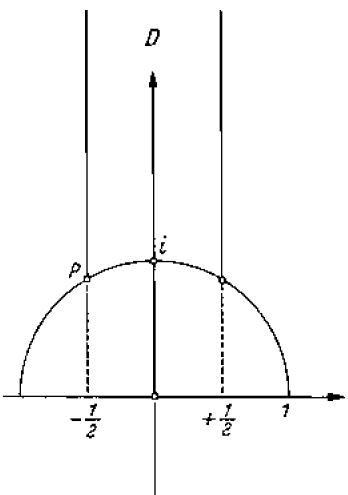
\includegraphics[width=0.42\linewidth]{figures/ch2-fundamental-domain.jpg}
  \label{fig:II-domain}
\end{figure}

\begin{proposition}\label{prop:II-4}
The stability group of $\rho=e^{2\pi i/3}$ (resp.\ of $i$) is of order
$3$ (resp.\ of order $2$), and is generated by $Q=ST$ (resp.\ by $S$).
Conversely, any point of $E$ with a non-trivial stability group is
equivalent under $G$ to either $\rho$ or $i$.
\end{proposition}

These three propositions will be proved at the same time. If
$w'=Aw=\frac{aw+b}{cw+d}$, a simple computation shows that:
\[
\operatorname{Im}(w')=\operatorname{Im}(w)/|cw+d|^{2}.
\tag{1}\label{eq:II-1}
\]

For a fixed $w\in E$, the set of all $cw+d$ ($c,d\in\mathbb{Z}$) is
discrete; hence, the $\operatorname{Im}(w')$ have no non-zero accumulation
point. Let then $G'$ be the subgroup of $G$ generated by $S$ and $T$, and
let $G'w$ be any orbit of $G'$ in $E$. By the above, we can assume that
$\operatorname{Im}(w)$ is maximum on $G'w$; formula \eqref{eq:II-1},
applied with $A=S$, gives $|w|\geq 1$. On the other hand,
$|\operatorname{Re}(T^{n}w)|\leq\frac{1}{2}$ for a suitable
$n\in\mathbb{Z}$; since $T$ does not change imaginary parts,
$\operatorname{Im}(T^{n}w)=\operatorname{Im}(w)$, and therefore
$T^{n}w\in D$. Thus, every orbit of $G'$ meets $D$.

Let now $w$ and $w'=Aw$ $(A\in G,\ A\neq 1)$ be points of $D$, with
$\operatorname{Im}(w')\geq\operatorname{Im}(w)$. Formula \eqref{eq:II-1}
then yields $|cw+d|\leq 1$, and, since we can assume $c\geq 0$, it follows
that $c=0$, $1$. If $c=0$, then $a=d=\pm 1$, $w'=w+b$, whence $b=\pm 1$
and $\operatorname{Re}w=\mp\frac{1}{2}$. If $c=1$, then we must have
$|w|=1$, $d=0$, unless $w$ is equal to $\rho$ or $\rho+1$, in which case
$d=0,1$ or $d=0,-1$. The formula $d=0$ gives
$w'=a-\frac{1}{w}=T^{a}Sw$. Since $Sw\in D$, the first part of the
discussion gives $a=0$, except when $\operatorname{Re}(Sw)=\pm\frac{1}{2}$,
i.e.\ $w=\rho$ or $\rho+1$; when $w=\rho$, one can take $a=-1$, and,
similarly for $w=\rho+1$. Finally, the formulas $w=\rho$, $d=1$ imply
$w'=a-1/(\rho+1)=a+\rho$, whence $a=0,1$.

Propositions \ref{prop:II-2} and \ref{prop:II-4} follow readily from this
discussion.

Let now $A\in G$, and let choose a point $w$ in the interior of $D$; the
orbit of $Aw$ under $G'$ meets $D$. Hence, there exists $B\in G'$ such
that $BAw\in D$. By propositions \ref{prop:II-2} and \ref{prop:II-4}, we
have $BA=1$, hence $A\in G'$, and proposition \ref{prop:II-3} is proved.

\subsection*{Remarks.}

\noindent
1) It is possible to prove (for instance, by topological arguments) that
the relations between $S$ and $T$ are generated by $(ST)^{3}=1$. Hence,
the modular group $G$ is isomorphic to the free product of a cyclic group
of order $2$ (corresponding to $S$) and a cyclic group of order $3$
(corresponding to $ST$).

\medskip\noindent
2) Let $Q(x,y)=Ax^{2}+Bxy+Cy^{2}$ be a positive definite binary quadratic
form, with real coefficients. Such a form can be written:
\[
Q(x,y)=|xw_{1}+yw_{2}|^{2},
\]
for a suitable choice of $w_{1}$, $w_{2}$. Applying proposition
\ref{prop:II-2} to $w=w_{1}/w_{2}$, one then obtains the existence of a
form $Q'=A'x^{2}+B'xy+C'y^{2}$ which is equivalent to $Q$ under the group
$\mathrm{SL}(2,\mathbb{Z})$, and verifies the inequalities:
\[
A'\geq C'\geq|B'|.
\]
[This ``reduction'' process was already given in Gauss's
\emph{Disquisitiones arithmeticae}.]

% ---------------------------------------------------------------
\section{Analytic structure and compactification of X=E/G}\label{sec:II-analytic}

We will first prove that the group $G$ is ``discontinuous'' in $E$:

\begin{proposition}\label{prop:II-5}
Let $K$ be a compact subset of $E$. Then:

(i) There exists a number $N$ such that $\operatorname{Im}(Aw)<N$ for
every $A\in G$ and $w\in K$.

(ii) For every compact subset $K'$ of $E$, the set of $A\in G$ such that
$AK\cap K'\neq\emptyset$ is finite. [i.e.\ $\lim AK=\infty$].
\end{proposition}

Statement (i) follows from formula \eqref{eq:II-1} and the fact that
$\inf|cw+d|>0$, when $w$ runs through $K$, and $c,d$ run through all pairs
of relatively prime integers.

Statement (ii) does in fact hold for every discrete subgroup of
$\mathrm{SL}(2,\mathbb{R})/\{\pm 1\}$. In the case of the modular group
$G$, it can be checked in the following way:

Formula \eqref{eq:II-1} shows that the number of pairs $(c,d)$ associated
with transformations $A\in G$ such that $AK\cap K'\neq\emptyset$ is
finite. But two elements $A_{1},A_{2}\in G$ have the same $(c,d)$ if and
only if $A_{1}=T^{n}A_{2}$ with some $n\in\mathbb{Z}$. Since
$T^{n}A_{2}K$ tends to $\infty$ with $n$, one has
$T^{n}A_{2}K\cap K'\neq\emptyset$ only for a finite number of values of
$n$, and (ii) follows immediately.

\begin{corollary}\label{cor:II-hausdorff}
The factor space $X=E/G$ is Hausdorff (and hence locally compact).
\end{corollary}

This is a formal consequence of (ii):

Let $w$ and $w'$ in $E$ be inequivalent under $G$. Since $Aw'\to\infty$,
there exists a compact neighbourhood $U$ of $w$ such that $Aw'\notin U$
for any $A\in G$. Let $V$ be a compact neighbourhood of $w'$ and
$N\subset G$ be the set of all $A$ such that $AV\cap U\neq\emptyset$; by
(ii), the set $N$ is finite. For any $A\in N$, let $W_{A}$ be a
neighbourhood of $Aw'$ which does not meet $U$, and put
$U'=V\cap\bigcap_{A\in N}A^{-1}W_{A}$; the set $U'$ is a neighbourhood of
$w'$. If $A\in N$, one has $AU'\subset W_{A}$ hence
$AU'\cap U=\emptyset$; if $A\notin N$, one has $AU'\subset AV$ hence again
$AU'\cap U=\emptyset$. This means that $GU$ and $GU'$ are disjoint
saturated neighbourhoods of the orbits $Gw$ and $Gw'$, q.e.d.

\begin{corollary}\label{cor:II-proper}
The canonical projection of the fundamental domain $D$ onto $X$ is proper.
\end{corollary}

If $K$ is a compact subset of $E$, one has to show that
$B=\bigcup_{A\in G}AK\cap D$ is compact. Property (ii) shows that
$\bigcup AK$ is locally finite, hence closed; on the other hand, property
(i) shows that $\operatorname{Im}(w)$ is bounded for $w\in B$. The set
$B$, being closed and bounded, is therefore compact.

\begin{corollary}\label{cor:II-homeo}
Let $R$ be the equivalence relation induced on $D$ by the equivalence
under $G$ (the relation $R$ has been given explicitly in prop.\
\ref{prop:II-2}). The canonical projection $D\to X$ induces an
homeomorphism of $D/R$ onto $X$.
\end{corollary}

The map $D/R\longrightarrow X$ is bijective (prop.~\ref{prop:II-2}),
continuous, and proper (follows from cor.~\ref{cor:II-proper}). Since both
$D/R$ and $X$ are locally compact, it is a homeomorphism.

After these preliminaries, we define an analytic structure on $X$ in the
following way:

Let $p:E\longrightarrow X$ denote the canonical projection. A continuous
function $f$ on an open set $U$ of $X$ is said to be holomorphic if
$f\circ p$ is holomorphic on $p^{-1}(U)$. One checks easily that the
axioms of a complex analytic structure are verified: if $P\in E$ is a
point of order $e$ (i.e.\ the stability group $G_{P}$ of $P$ is of order
$e$), we can find a local parameter $z_{P}$ around $P$ such that $G_{P}$
operates on $z_{P}$ by multiplication by $e$-th roots of unity, and
$(z_{P})^{e}$ is a local parameter around $p(P)\in X$ [one can take for
instance $z_{P}=(w-P)/(w-\bar{P})$].

Let now $\hat{X}=X\cup\{\infty\}$ be the one-point compactification of
$X$; we now want to extend to $\hat{X}$ the analytic structure of $X$.
Let $E_{1}$ be the half plane $\operatorname{Im}(w)>1$; it follows from
formula \eqref{eq:II-1} that the equivalence relation induced on $E_{1}$
by $G$ is given by the translations $T^{n}$. One has therefore
$p(E_{1})\approx E_{1}/T$; but the mapping $w\longrightarrow
q=e^{2\pi iw}$ is an analytic isomorphism of $E_{1}/T$ onto some open disk
(minus the origin); putting $q(\infty)=0$, we then extend $q$ to
$p(E_{1})\cup\{\infty\}$, and take this function as a local parameter
around $\infty$ on $\hat{X}$. This gives the desired extension. A
meromorphic function on $\hat{X}$ may therefore be defined as a
meromorphic function on $E$, invariant under $G$, admitting a power series
expansion $\sum_{n\geq k}a_{n}q^{n}$ which converges around $q=0$. Such a
function is called a \emph{modular function}.

\begin{proposition}\label{prop:II-6}
The space $\hat{X}$ is analytically isomorphic to the sphere
$S_{2}=\hat{\mathbb{C}}$.
\end{proposition}

By cor.~\ref{cor:II-homeo} to prop.~\ref{prop:II-3}, $X$ is homeomorphic
to $D/R$, i.e.\ to a plane. The Riemann surface $\hat{X}$ is therefore
homeomorphic to $S_{2}$, and, as is well known, this implies that it is
analytically isomorphic to $S_{2}$.

If $\lambda:\hat{X}\longrightarrow\hat{\mathbb{C}}$ is an analytic
isomorphism, every modular function is a rational function of $\lambda$.
Such a $\lambda$ is determined up to an analytic automorphism of
$\hat{\mathbb{C}}$; we normalize it by asking that it maps $\infty$ and
$p(\rho)$ on-to $\infty$ and $0$ respectively, and has residue equal to
$1$ at $\infty$ (when expanded in a power series of $q$). This particular
choice of $\lambda$ will be referred to as ``the'' modular function, and
be denoted by $j$.

\noindent\emph{Note.} Proposition \ref{prop:II-6} means that $X$ is
analytically isomorphic to $\mathbb{C}$. This can also be proved by using
the fact that the ``half fundamental domain''
$D_{+}=\{w\mid 0<\operatorname{Re}w<\frac{1}{2},\ |w|>1\}$ is analytically
isomorphic to a half plane, and applying Schwarz's symmetry principle.

% ---------------------------------------------------------------
\section{Modular functions of weight k}\label{sec:II-weight}

A (meromorphic) modular function of weight $k$ ($k\in\mathbb{Z}$) is a
meromorphic function $h$ on $E$ such that:
\[
h(Aw)=(cw+d)^{2k}h(w)\qquad(A\in G),
\tag{2}\label{eq:II-2}
\]
and which admits a Laurent expansion in $q=e^{2\pi iw}$ with a finite
number of negative exponents:
\[
h=\sum\nolimits_{n\geq k}a_{n}q^{n}.
\]

A function of weight $0$ is thus a modular function in the sense of
§\ref{sec:II-analytic}. A modular function of weight $k$ which is
holomorphic in $E$ and at $\infty$ is called a \emph{modular form}.

Equation \eqref{eq:II-2} is equivalent to the fact that the function of
$w_{1},w_{2}$ defined by:
\[
h(w_{1},w_{2})=w_{2}^{-2k}h(w_{1}/w_{2})
\]
is invariant under the group $\mathrm{SL}(2,\mathbb{Z})$; note that
$h(w_{1},w_{2})$ is homogeneous of degree $-2k$.

Since $d\bigl(\frac{aw+b}{cw+d}\bigr)=dw/(cw+d)^{2}$, one can also express
\eqref{eq:II-2} by saying that the differential form of degree $k$
$\omega=h\,dw^{k}$ is invariant by $G$, and hence represents a differential
form on $\hat{X}$. The condition that $h$ be meromorphic on $E$ and at
$\infty$ means that $\omega$ is everywhere meromorphic on $\hat{X}$. More
precisely:

\begin{proposition}\label{prop:II-7}
Let $\omega=h\,dw^{k}$ be the differential form on $\hat{X}$ associated
with the modular function $h$ of weight $k$. For any point $P\in E$, let
$w_{P}(h)$ denote the order of $h$ at $P$ and $v_{P}(\omega)$ the order of
$\omega$ at the corresponding point of $\hat{X}$; let $w_{\infty}(h)$ and
$v_{\infty}(\omega)$ be defined similarly. Then:
\[
w_{\infty}(h)=v_{\infty}(\omega)+k,
\tag{3}\label{eq:II-3}
\]
\[
w_{P}(h)=e\cdot v_{P}(\omega)+k(e-1)\qquad(e=\text{order of }P).
\tag{4}\label{eq:II-4}
\]
\end{proposition}

Equation \eqref{eq:II-3} follows immediately from the relation
$2\pi i\,dw=\frac{dq}{q}$. For $P\in E$, choose a local parameter $z_{P}$
such that the isotropy group $G_{P}$ operates on $z_{P}$ by multiplication
by $e$-th roots of unity, and let $t=(z_{P})^{e}$. We can then write:
\[
\begin{gathered}
\omega=u\,t^{N}dt^{k}\quad(u\ \text{holomorphic}\neq 0,\ N=v_{P}(\omega)),\\
\omega=u\,e^{k}(z_{P})^{Ne+k(e-1)}(dz_{P})^{k},
\end{gathered}
\]
which yields \eqref{eq:II-4}.

On an algebraic curve of genus $g$, the sum of the orders of a
differential form of degree $k$ is equal to $k(2g-2)$. Here $g=0$. Hence:

% 原书中命题 7 的两条推论编号重新从 1 开始（Corollary 1, 2）。
\setcounter{corollary}{0}
\xdef\theHcorollary{ch2.blockB.\arabic{corollary}}
\begin{corollary}\label{cor:II-valence}
If $h$ is a modular function of weight $k$, one has:
\[
w_{\infty}(h)+\frac{1}{2}w_{i}(h)+\frac{1}{3}w_{\rho}(h)
+\Sigma^{*}\,w_{P}(h)=\frac{k}{6},
\tag{5}\label{eq:II-5}
\]
where $\Sigma^{*}$ means that $P$ runs through a set of representatives
of the equivalence classes of ordinary points (i.e.\ points of order $1$).
\end{corollary}

\noindent[Formula \eqref{eq:II-5} can also be proved directly by
integrating $dh/h$ over the boundary of $D$.]

Let $M_{k}$ denote the vector space of modular forms of weight $k$. If $h$
is a non-zero element of $M_{k}$, one has $w_{P}(h)\geq 0$ for all
$P\in E$ and also $w_{\infty}(h)\geq 0$. Formula \eqref{eq:II-5} then
shows that $k\geq 0$. For $k=0$, the only elements of $M_{k}$ are the
constants; for $k=1$, formula \eqref{eq:II-5} shows that $M_{k}=0$. For
$k=2$, one sees that every non-zero element $h\in M_{k}$ has a zero only
on the orbit of $\rho$, and that these zeros are simple; if $h'\in M_{2}$,
a suitable linear combination $h'-ah$ has a zero outside this orbit, hence
is identically zero; this shows that $\dim M_{2}\leq 1$. An analogous
result holds for $M_{3}$ with $i$ replacing $\rho$. We have proved:

\begin{corollary}\label{cor:II-dim}
a) $M_{k}=0$ for $k<0$ and for $k=1$.

b) $\dim M_{k}\leq 1$ for $k=2,3$.

c) If $h$ is a non-zero element of $M_{2}$ (resp.\ $M_{3}$), it has zeros
only on the orbit of $\rho$ (resp.\ of $i$), and these zeros are simple.
\end{corollary}

% ---------------------------------------------------------------
\section{Eisenstein series}\label{sec:II-eisenstein}

Let $\Gamma=\mathbb{Z}w_{1}+\mathbb{Z}w_{2}$ be a lattice in
$\mathbb{C}$, and let $k$ be an integer, with $k\geq 2$. The Eisenstein
series $G_{k}(\Gamma)$ of degree $k$ associated to $\Gamma$ is defined by
the formula:
\[
G_{k}(\Gamma)=\sum_{u\in\Gamma-\{0\}}\frac{1}{u^{2k}}
=\!\!\sum_{\substack{m,n\in\mathbb{Z}\\(m,n)\neq(0,0)}}\!\!
(mw_{1}+nw_{2})^{-2k}.
\tag{6}\label{eq:II-6}
\]

The series $G_{2}$ and $G_{3}$ are identical (up to a constant factor)
with the $g_{2}$ and $g_{3}$ of Weierstrass's theory:
\[
g_{2}=60\,G_{2},\qquad g_{3}=140\,G_{3}.
\]

To the homogeneous function $G_{k}(w_{1},w_{2})=G_{k}(\Gamma)$ is
associated a function $G_{k}(w)$ of $w=w_{1}/w_{2}$ by the formula:
\[
G_{k}(w)=(w_{2})^{2k}G_{k}(w_{1},w_{2})
=\sum_{\substack{m,n\in\mathbb{Z}\\(m,n)\neq(0,0)}}(m+nw)^{-2k}.
\tag{8}\label{eq:II-8}
\]

\begin{proposition}\label{prop:II-8}
For $k\geq 2$, the series \eqref{eq:II-8} is absolutely convergent in $E$
and normally convergent in $D$. Its sum $G_{k}(w)$ is a modular form of
weight $k$ whose value at infinity is equal to $2\zeta(2k)$.
\end{proposition}

In $D$, we have $|\operatorname{Re}(w)|\leq\frac{1}{2}$ and
$|w|\geq 1$, whence:
\[
|m+nw|^{2}\geq m^{2}-nm+n^{2},
\]
which is a positive definite quadratic form. This implies the normal
convergence of \eqref{eq:II-8} in $D$, hence its absolute convergence in
$E$. The fact that $G_{k}(w_{1},w_{2})$ is invariant by
$\mathrm{SL}(2,\mathbb{Z})$ implies that $G_{k}(w)$ verifies
\eqref{eq:II-2}. When $w$ tends to infinity in $D$, each term
$(m+nw)^{-2k}$, $n\neq 0$, tends to zero, and $G_{k}(w)$ tends to
$\sum_{m\neq 0}m^{-2k}=2\zeta(2k)$; hence $G_{k}(w)$ is a modular form.

Let now $\Delta=g_{2}^{3}-27g_{3}^{2}$. It is clear that $\Delta$ is a
modular form of weight $6$; since $g_{2}(\rho)=0$ and $g_{3}(\rho)\neq 0$
(cor.~\ref{cor:II-dim} to prop.~\ref{prop:II-7}), one has
$\Delta(\rho)\neq 0$ and $\Delta$ is not identically zero. On the other
hand:
\[
\begin{aligned}
g_{2}(\infty)&=60\,G_{2}(\infty)=120\,\zeta(4)=120\pi^{4}/90=\tfrac{4}{3}\pi^{4}\\
g_{3}(\infty)&=140\,G_{3}(\infty)=280\,\zeta(6)=560\pi^{6}/945=\tfrac{8}{27}\pi^{6},
\end{aligned}
\]
hence $\Delta(\infty)=0$. Formula \eqref{eq:II-5} then shows that
$w_{\infty}(\Delta)=1$ and that $\Delta$ is everywhere $\neq 0$ on $E$.

\begin{proposition}\label{prop:II-9}
Let $\varepsilon:M_{k}\longrightarrow\mathbb{C}$ be the homomorphism
$h\longrightarrow h(\infty)$, and $\Delta:M_{k-6}\longrightarrow M_{k}$ be
the multiplication by $\Delta$. For $k\geq 2$ the sequence:
\[
0\rightarrow M_{k-6}\xrightarrow{\ \Delta\ }M_{k}
\xrightarrow{\ \varepsilon\ }\mathbb{C}\rightarrow 0
\]
is exact.
\end{proposition}

Since $\varepsilon(G_{k})=2\zeta(2k)\neq 0$, $\varepsilon$ is surjective.
If now $\varepsilon(h)=0$, then the function $h/\Delta$ is holomorphic in
$E$ (since $\Delta\neq 0$ on $E$), holomorphic at $\infty$ (since
$w_{\infty}(\Delta)=1$), and of weight $k-6$, hence belongs to $M_{k-6}$.

\begin{corollary}\label{cor:II-dimMk}
For $k\geq 2$, the dimension of the space $M_{k}$ is given by:
\[
\dim M_{k}=
\begin{cases}
[k/6] & \text{if } k\equiv 1\bmod 6\\
[k/6]+1 & \text{if } k\not\equiv 1\bmod 6.
\end{cases}
\]
\end{corollary}

Proof by induction on $k$, using cor.~\ref{cor:II-dim} to
prop.~\ref{prop:II-7}.

\begin{corollary}\label{cor:II-isobaric}
Every modular form is an isobaric polynomial in $g_{2}$ and $g_{3}$.
\end{corollary}

Let $k\geq 2$. There exist positive integers $a,b$ such that
$2a+3b=k$; the form $g_{2}^{b}g_{3}^{a}$ belongs to $M_{k}$, and
$\varepsilon(g_{2}^{b}g_{3}^{a})\neq 0$. Prop.~\ref{prop:II-9} then shows
that every element $h\in M_{k}$ may be written
\[
h=\lambda\,g_{2}^{b}g_{3}^{a}+\Delta h',\qquad\text{with }h'\in M_{k-6},
\]
and our contention follows by induction on $k$.

\subsection*{Remark.}
Cor.~\ref{cor:II-dimMk} can also be obtained by the following argument:
Let $P$ (resp.\ $Q,R$) denote the point at infinity (resp.\ the image of
$i$, $\rho$) in $\hat{X}$. Proposition \ref{prop:II-7} shows that $M_{k}$
is canonically isomorphic with the vector space $\Omega_{k}$ of
differential forms $\omega$ of degree $k$ on $\hat{X}$ whose divisors
$(\omega)$ verify:
\[
(\omega)\geq-kP-[k/2]\,Q-[2k/3]\,R.
\tag{9}\label{eq:II-9}
\]
If $K$ denotes the canonical class of $\hat{X}$, $\Omega_{k}$ is in turn
isomorphic with $L(D_{k})$, with
$D_{k}=kK+kP+[k/2]Q+[2k/3]R$. If $k\geq 2$, one has
$\deg(D_{k})=-k+[k/2]+[k/3]\geq -1$, and the Riemann--Roch formula
(applied here to a curve of genus zero!) gives:
\[
\dim M_{k}=\dim L(D_{k})=\deg(D_{k})+1=1-k+[k/2]+[2k/3],
\]
an expression which is easily seen to be equivalent to
cor.~\ref{cor:II-dimMk}.

This interpretation of $M_{k}$ (which applies as well to other
discontinuous groups than the modular group) can also be used to derive
explicit formulas for the $G_{k}$ in terms of $j$. One gets for instance:
\[
g_{2}\,dw^{2}=-\frac{\pi^{2}}{3}\frac{dj^{2}}{j(j-2^{6}3^{3})},\qquad
g_{3}\,dw^{3}=\frac{\pi^{3}}{27i}\frac{dj^{3}}{j^{2}(j-2^{6}3^{3})}.
\tag{10}\label{eq:II-10}
\]

% ---------------------------------------------------------------
\section{\texorpdfstring{The q-expansions of $G_{k}$, $\Delta$ and
$j$}{The q-expansions of Gk, Delta and j}}\label{sec:II-qexp}

If $n$ is an integer $\geq 1$ and $s$ any number, we put:
\[
\sigma_{s}(n)=\sum_{d\mid n}d^{s}.
\]

\begin{proposition}\label{prop:II-10}
The q-expansion of $G_{k}$, $k\geq 2$, is:
\[
G_{k}=2\zeta(2k)+2\,(2\pi)^{2k}(-1)^{k}/(2k-1)!
\sum_{n=1}^{\infty}\sigma_{2k-1}(n)\,q^{n}.
\tag{11}\label{eq:II-11}
\]
\end{proposition}

We start from the equality:
\[
\sum_{m\in\mathbb{Z}}(m+w)^{-2}=\pi^{2}/\sin^{2}\pi w
=(2\pi i)^{2}\sum_{n=1}^{\infty}nq^{n}\qquad(q=e^{2\pi iw}).
\]

Taking successive derivatives with respect to $w$, we get:
\[
(s-1)!\sum_{m\in\mathbb{Z}}(m+w)^{-s}
=(-2\pi i)^{s}\sum_{n=1}^{\infty}n^{s-1}q^{n}.
\]

On the other hand, we have:
\[
G_{k}=2\zeta(2k)+2\sum_{n=1}^{\infty}\sum_{m\in\mathbb{Z}}(m+nw)^{-2k}.
\tag{12}\label{eq:II-12}
\]

Combined with \eqref{eq:II-12}, this gives
\[
G_{k}=2\zeta(2k)+2\,(-2\pi i)^{2k}/(2k-1)!
\sum_{\substack{d\geq 1\\ n\geq 1}}d^{2k-1}q^{dn},
\]
hence \eqref{eq:II-11}.

\begin{proposition}\label{prop:II-11}
We have $\Delta=(2\pi)^{12}q(1+a_{1}q+\dots)$ and
$j=q^{-1}+b_{0}+b_{1}q+\dots$, where the $a_{i}$'s and the $b_{i}$'s are
rational integers. Moreover, $j$ is equal to $2^{6}3^{3}g_{2}^{3}/\Delta$.
\end{proposition}

Let us put $U=\sum_{n=1}^{\infty}\sigma_{3}(n)q^{n}$ and
$V=\sum_{n=1}^{\infty}\sigma_{5}(n)q^{n}$.

Prop.~\ref{prop:II-10} then shows that:
\[
\left\{
\begin{aligned}
g_{2}&=60\,G_{2}=(2\pi)^{4}\tfrac{1}{2^{2}\cdot 3}\,(1+240U)\\
g_{3}&=140\,G_{3}=(2\pi)^{6}\tfrac{1}{2^{3}\cdot 3^{3}}\,(1-504V)
\end{aligned}\right.
\tag{13}\label{eq:II-13}
\]
hence:
\[
\Delta=(2\pi)^{12}\tfrac{1}{2^{6}\cdot 3^{3}}
\bigl[(1+240U)^{3}-(1-504V)^{2}\bigr].
\tag{14}\label{eq:II-14}
\]

The fact that the $a_{i}$'s are integers is therefore equivalent to the
congruence
\[
(1+240U)^{3}\equiv(1-504V)^{2}\quad\bmod\ 2^{6}\,3^{3}.
\tag{15}\label{eq:II-15}
\]

A little calculation shows that \eqref{eq:II-15} is in turn equivalent to
the congruence $U\equiv V\bmod 2^{2}3$, or
$\sigma_{3}(n)\equiv\sigma_{5}(n)\bmod 2^{2}3$; this last congruence is a
trivial consequence of $d^{3}\equiv d^{5}\bmod 2^{2}3$. This proves our
assertion on $\Delta$.

The function $g_{2}^{3}/\Delta$ is a modular function which is holomorphic
on $E$ and has a simple pole at infinity. Hence
$g_{2}^{3}/\Delta=aj+b$, with $a,b\in\mathbb{C}$. Since
$g_{2}(\rho)=j(\rho)=0$, one has $b=0$. One the other hand
$g_{2}(\infty)=4\pi^{4}/3$, and therefore the coefficient of $q^{-1}$ in
the q-expansion of $g_{2}^{3}/\Delta$ is equal to $2^{-6}3^{-3}$. Since
the corresponding coefficient of $j$ is equal to $1$ (by definition), this
gives $a=2^{-6}3^{-3}$, and $j=2^{6}3^{3}g_{2}^{3}/\Delta$.

We then have:
\[
j=(1+240U)^{3}q^{-1}(1+a_{1}q+\dots)^{-1},
\]
and since the $a_{i}$'s and the coefficients of $U$ are in
$\mathbb{Z}$, so are the coefficients of $j$, q.e.d.

\begin{proposition}[``q-expansion principle'']\label{prop:II-qprin}
Let $f=\sum_{n\geq N}x_{n}q^{n}$ be a modular function which is
holomorphic in $E$ and has a pole of order $N$ at infinity. Then $f$ is a
polynomial in $j$ of degree $N$:
\[
f=\sum_{n=0}^{n=N}y_{n}j^{n}.
\]
Moreover, the additive subgroup $A$ of $\mathbb{C}$ generated by the
$x_{n}$'s is the same as the additive subgroup $B$ generated by the
$y_{n}$'s.
\end{proposition}

If $N=0$, $f=x_{0}$ and $A=B=\mathbb{Z}x_{0}$. If $N>0$, put
$g=f-x_{-N}j^{N}$. The function $g$ has a pole of order $\leq N-1$ at
infinity, and may then be written:
\[
g=\sum\nolimits_{n<N}y_{n}j^{n}.
\]
One has $f=g+x_{-N}j^{N}$, which shows that $B(f)$ is the subgroup of
$\mathbb{C}$ generated by $B(g)$ and $x_{-N}$. On the other hand, the
fact that $j$ has integral coefficients shows that $A(f)$ is also
generated by $A(g)=B(g)$ and $x_{-N}$, q.e.d.

% ---------------------------------------------------------------
\section{Explicit formula for the q-expansion of Delta}\label{sec:II-delta}

This formula will not be needed to prove the main results on complex
multiplication outlined in chapter I. However, since it is of considerable
interest in itself (Ramanujan's function!), we give here a proof of it.
We will essentially follow Hurwitz (Math.\ Werke, Bd.\ I, S.~1--67,
578--595).

\begin{proposition}\label{prop:II-13}
One has $\displaystyle\Delta=(2\pi)^{12}q\prod_{n=1}^{\infty}(1-q^{n})^{24}$.
\end{proposition}

The product $f=q\prod_{n=1}^{\infty}(1-q^{n})^{24}$ is a holomorphic
function on $E$, invariant by the translation $T$, and holomorphic at
infinity. It is enough to prove it is of weight $6$, since prop.~%
\ref{prop:II-9} will then show that it is equal to $\lambda\Delta$, and
the factor $\lambda$ will be determined by looking at the coefficient of
$q$. By prop.~\ref{prop:II-3}, we then have to show that
\[
f(-1/w)=w^{12}f(w)\qquad\text{for }w\in E.
\tag{16}\label{eq:II-16}
\]

Since $f$ does not vanish on $E$, one can pick up a determination of
$f^{1/24}$, for instance:
\[
\eta=e^{\pi iw/12}\prod_{n=1}^{\infty}(1-e^{2\pi inw}).
\]

The function $\eta$ is holomorphic on $E$, and \eqref{eq:II-16} is
equivalent to
\[
\eta(-1/w)=\sqrt{w/i}\;\eta(w)\,.
\tag{17}\label{eq:II-17}
\]

The rest of this section is devoted to the proof of \eqref{eq:II-17}. For
another proof, see for instance C.L. Siegel, Mathematika, 1, p.~4.

\begin{lemma}\label{lem:II-1}
The series $G_{1}(w)=\sum_{n}\bigl[\sum_{m}(m+nw)^{-2}\bigr]$ converges
absolutely and one has $G_{1}(w)\,dw=-4\pi i\,d\eta/\eta$.
\end{lemma}

(As usual, one removes the term corresponding to $(n,m)=(0,0)$.) Using
again the formula $\pi^{2}/\sin^{2}\pi nw=\sum_{m}(m+nw)^{-2}$, we get the
absolute convergence in $m$ (for fixed $n$), and the formula:
\[
\begin{aligned}
G_{1}(w)
&=2\,\zeta(2)+2\sum_{n=1}^{\infty}\pi^{2}/\sin^{2}\pi nw\\
&=\pi^{2}/3-8\pi^{2}\sum_{n=1}^{\infty}q^{n}/(1-q^{n})^{2},
\end{aligned}
\]
whence the absolute convergence in $n$.

This can be written:
\[
G_{1}(w)\,dw=(\pi/6i)\bigl(1-24\sum_{n=1}^{\infty}\sum_{m=1}^{\infty}
nq^{nm}\bigr)dq/q.
\]

On the other hand:
\[
\begin{aligned}
d\eta/\eta
&=dq/24q-\sum_{n=1}^{\infty}nq^{n-1}dq/(1-q^{n})\\
&=(dq/24q)\bigl(1-24\sum_{n=1}^{\infty}\sum_{m=1}^{\infty}nq^{nm}\bigr),
\end{aligned}
\]
whence the lemma.

\begin{lemma}\label{lem:II-2}
We have:
\[
\sum_{m}\Bigl[\sum_{n}(m-1+nw)^{-1}(m+nw)^{-1}\Bigr]=-2\pi i/w,
\tag{18}\label{eq:II-18}
\]
\[
\sum_{n}\Bigl[\sum_{m}(m-1+nw)^{-1}(m+nw)^{-1}\Bigr]=0,
\tag{19}\label{eq:II-19}
\]
where the series are absolutely convergent.
\end{lemma}

(As before, we remove the terms $(n,m)=(0,0),(0,1)$.)

Let us denote by $H$ (resp.\ $H_{1}$) the left side of \eqref{eq:II-18}
(resp.\ of \eqref{eq:II-19}).

It is clear that the first summations are absolutely convergent. The formula:
\[
(m-1+nw)^{-1}(m+nw)^{-1}=(m-1+nw)^{-1}-(m+nw)^{-1}
\]
gives:
\[
\begin{aligned}
\sum
olimits_{n}(m-1+nw)^{-1}(m+nw)^{-1}
&=\lim_{n\to\infty}\sum_{-n}^{n}\bigl[(m-1+nw)^{-1}-(m+nw)^{-1}\bigr]\\
&=(\pi/w)\bigl(\cot\pi\tfrac{m-1}{w}-\cot\pi\tfrac{m}{w}\bigr),
\end{aligned}
\]
with the convention $\cot a/w=0$ if $a=0$.

We then have:
\[
H=(\pi/w)\sum_{m}\bigl(\cot\pi\tfrac{m-1}{w}-\cot\pi\tfrac{m}{w}\bigr),
\]
a series which is easily proved to be absolutely convergent. Its sum is
given by:
\[
\begin{aligned}
H
&=(\pi/w)\lim_{m\to\infty}\sum_{-m}^{m}\bigl(\cot\pi\tfrac{m-1}{w}
 -\cot\pi\tfrac{m}{w}\bigr)\\
&=(\pi/w)\lim_{m\to\infty}\bigl(\cot\pi\tfrac{m+1}{w}+\cot\pi\tfrac{m}{w}\bigr)
=-2\pi i/w,
\end{aligned}
\]
since $\cot\pi\frac{m}{w}$ tends to $i$ when $m$ tends to infinity.

On the other hand, we have:
\[
\begin{aligned}
\sum
olimits_{m}(m-1+nw)^{-1}(m+nw)^{-1}
&=\lim_{m\to\infty}\sum_{-m}^{m}\bigl((m-1+nw)^{-1}-(m+nw)^{-1}\bigr)\\
&=\lim_{m\to\infty}\bigl((-m-1+nw)^{-1}-(m+nw)^{-1}\bigr)=0,
\end{aligned}
\]
whence $H_{1}=0$.

\begin{lemma}\label{lem:II-3}
We have $G_{1}(-1/w)=w^{2}G_{1}(w)-2\pi iw$.
\end{lemma}

Let us put
\[
G(w)=\sum_{m}\sum_{n}(m+nw)^{-2}.
\]

We have:
\[
H_{1}-G_{1}=\sum_{n}\sum_{m}(m+nw)^{-2}(m-1+nw)^{-1},
\]
which is absolutely convergent (as a double series). We can then
interchange the order of summations, and we get:
\[
H_{1}-G_{1}=H-G.
\]
Using lemma \ref{lem:II-2}, we have then $G_{1}(w)-G(w)=2\pi i/w$. Using
the obvious formula:
\[
G_{1}(-1/w)=w^{2}G(w),
\]
we obtain lemma \ref{lem:II-3}.

\subsection*{Proof of \texorpdfstring{\eqref{eq:II-17}}{(17)}.}

Lemma \ref{lem:II-3} may be written:
\[
G_{1}(-1/w)\cdot d(-1/w)=G_{1}(w)\,dw-2\pi i\,dw/w.
\]
Using lemma \ref{lem:II-1}, this gives:
\[
(d\eta/\eta)(-1/w)=d\eta/\eta+dw/2w,
\]
which means that
\[
\eta(-1/w)=C\,w^{1/2}\,\eta(w).
\]
Putting $w=1$ gives $C\sqrt{i}=1$, and \eqref{eq:II-17} is proved.
